\section{Distributed and point input to a segment}
In general, segments receive distributed and point sources of
input each of which require a different mathematical treatment.
The current supplied by distributed input such as intrinsic
voltage-dependent current or capacitative current is proportional
to the surface area of the segment on which it acts, whereas the
current supplied to a segment at a synapse or by an exogenous
point input is independent of the size of the segment. An implicit
assumption of a compartmental model is that distributed current
input to a segment is small by comparison with axial current
flowing along the segment.

To appreciate why this assumption is reasonable, consider a
cylindrical dendritic segment of radius $r$ (cm), length $h$ and
with membrane of constant conductance $g_\mathrm{M}$ (mS/cm$^2$).
Suppose that axoplasm has constant conductance $g_\mathrm{A}$
(mS/cm) and that a potential difference $V$ (mV) exists between
the segment boundaries, then the axial current along the segment
is $I_\mathrm{A}=\pi r^2 g_\mathrm{A} V/h$ ($\mu$A) and the total
distributed current crossing the membrane of the segment is
$I_\mathrm{M}=2\pi r h g_\mathrm{M}\,(V/2)$. The ratio of the
distributed current to the axial current is therefore
\begin{equation}\label{pc1}
\frac{\mbox{Distributed current}}{\mbox{Axial current}}
=\frac{I_\mathrm{M}}{I_\mathrm{A}}=\frac{\pi r h g_\mathrm{M}\,V}
{\pi r^2 g_\mathrm{A}\,(V/h)}=\frac{h^2 g_\mathrm{M}} {r
g_\mathrm{A}}=\Big(\frac{h}{r}\Big)^2\, \frac{r
g_\mathrm{M}}{g_\mathrm{A}}\,.
\end{equation}
For a typical dendritic segment $r g_\mathrm{M}/g_\mathrm{A}$ is
small (say $ \approx 10^{-5}$), and therefore distributed current
acting on a segment is small by comparison with axial current for
``short'' segments. On the other hand, segments several orders of
magnitude longer than their radius can be expected to have
distributed and axial currents of similar magnitude. An important
property of a compartmental model is that segments are not
excessively long by comparison with their radius. In the treatment
of distributed current, the development of the new compartmental
model makes explicit use of the assumption that distributed
current is much smaller than axial current. Since this assumption
may not be valid for point sources of current, it will not be made
for the treatment of these current in the new compartmental model.

\subsection{Axial current in the absence of distributed and point current input}
Figure \ref{model} illustrates a dendritic segment of length $h$
(cm) where $\lambda\in[0,1]$ is the fractional distance of a point
of the segment from its proximal end ($\lambda=0$). Let
$r_\mathrm{P}$ and $r_\mathrm{D}$ be the radii of the segment at
its proximal and distal boundaries respectively, let
$V_\mathrm{P}(t)$ and $V_\mathrm{D}(t)$ be the membrane potentials
at these boundaries and let $I_\mathrm{PD}$ be the axial current
in the segment in the absence of transmembrane current.

\begin{figure}[!h]
\centering
\begin{tabular}{c}
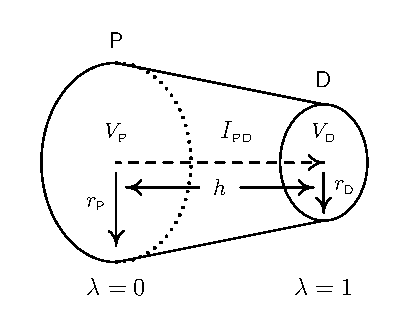
\includegraphics[ ]{NewCompFig2.eps}
\end{tabular}\qquad
\begin{tabular}{p{2.55in}}
\caption{\label{model} A segment of length $h$ (cm) is illustrated. In
the absence of transmembrane current, membrane potentials $V_\mathrm{P}$
and $V_\mathrm{D}$ at the proximal and distal boundaries of the
segment generate axial current $I_\mathrm{PD}$.}
\end{tabular}
\end{figure}

%\begin{figure}[!h]
%\centering
%\begin{tabular}{c}
%\begin{mfpic}[1][1]{-40}{140}{180}{300}
%\headlen7pt
%\pen{0.5pt}
%\dotspace=4pt
%\dotsize=1pt
%\pen{1pt}
%\dotspace=4pt
%\dotsize=1.5pt
%%
%% LH cylinder
%\parafcn[s]{-180,180,5}{(100-21*sind(t),240+28*cosd(t))}
%\lines{(0,288),(100,268)}
%\lines{(0,192),(100,212)}
%%
%% Partial cylinder on left
%\dotted\parafcn[s]{0,180,5}{(36*sind(t),240+48*cosd(t))}
%\parafcn[s]{0,180,5}{(-36*sind(t),240+48*cosd(t))}
%%
%% Annotation of LH cylinder
%\dashed\arrow\lines{(0,240),(100,240)}
%\tlabel[bl](50,250){\large $I_\mathrm{PD}$}
%\tlabel[bc](0,250){$V_\mathrm{P}$}
%\tlabel[cc](0,180){\large $\lambda=0$}
%\tlabel[bc](0,295){\textsf{P}}
%\arrow\lines{(0,235),(0,200)}
%\tlabel[cr](-5,220){\textsf{$r_\mathrm{P}$}}
%%
%% Annotation of RH cylinder
%\tlabel[bc](100,250){$V_\mathrm{D}$}
%\tlabel[cc](100,180){\large $\lambda=1$}
%\tlabel[cc](100,280){\textsf{D}}
%\arrow\lines{(100,235),(100,216)}
%\tlabel[cl](105,228){\textsf{$r_\mathrm{D}$}}
%\arrow\lines{(60,228),(95,228)}
%\arrow\lines{(40,228),(5,228)}
%\tlabel[cc](50,228){$h$}
%\end{mfpic}
%\end{tabular}\qquad
%\begin{tabular}{p{2.55in}}
%\caption{\label{model} A segment of length $h$ (cm) is illustrated. In
%the absence of transmembrane current, membrane potentials $V_\mathrm{P}$
%and $V_\mathrm{D}$ at the proximal and distal boundaries of the
%segment generate axial current $I_\mathrm{PD}$.}
%\end{tabular}
%\end{figure}

The membrane of the segment in Figure \ref{model} is formed by
rotating the straight line PD about the axis of the dendrite to
form the frustum of a cone of radius
\begin{equation}\label{mp1}
r(\lambda)=(1-\lambda)r_\mathrm{P}+\lambda r_\mathrm{D} \,,\qquad
\lambda\in[0,1]\,.
\end{equation}
Assuming that the segment is filled with axoplasm of
constant conductance $g_\mathrm{A}$ and that no current
crosses its membrane, then the relationship between
$V_\mathrm{P}$, $V_\mathrm{D}$ and $I_\mathrm{PD}$ can be
constructed by integrating
\[
I_\mathrm{PD}=-\frac{g_\mathrm{A}\pi}{h}\,\Big[\,
(1-\lambda)r_\mathrm{P}+\lambda r_\mathrm{D}\,\Big]^2\,
\frac{dV}{d\lambda}
\]
with boundary conditions $V(0)=V_\mathrm{P}$ and
$V(1)=V_\mathrm{D}$. This calculation shows that the potentials
$V_\mathrm{P}$ and $V_\mathrm{D}$ give rise to axial current
\begin{equation}\label{mp2}
I_\mathrm{PD}= \frac{\pi g_\mathrm{A} r_\mathrm{P}
r_\mathrm{D}}{h}\,\big(\,V_\mathrm{P}-V_\mathrm{D}\,\big)
\end{equation}
in the absence of distributed and point currents, and that the
potential at point $\lambda$ is
\begin{equation}\label{mp3}
V(\lambda) = \frac{V_\mathrm{P}\,(1-\lambda)\,
r_\mathrm{P}+V_\mathrm{D}\,\lambda\,r_\mathrm{D}}
{(1-\lambda)\,r_\mathrm{P}+\lambda\,r_\mathrm{D}}\,.
\end{equation}
Expressions (\ref{mp2}) and (\ref{mp3}) are estimates of the axial
current flowing along a segment and the potential distribution within
the segment in the absence of transmembrane current.

\subsection{Motivation for partitioning point current input - model
accuracy}\label{assertion}

One inescapable feature of a traditional compartmental model is
that small variations in the location of segment boundaries, as
might occur when a dendrite is represented by segments, may exert
a large influence on the solution of the resulting mathematical
model. Consider, for example, a point input close to a segment
boundary. A small variation in the position of that boundary may
change the assigned location of this input from the centre of one
segment to that of an adjacent segment. With respect to the
mathematical model, the location of this input is therefore
determined only to an accuracy of half a segment length, and this
indeterminacy will in turn generate a model solution that is
particularly sensitive to segment boundaries -- small changes in
these boundaries may lead to large changes in the model solution.
Of course, with a small number of point sources of input, this
problem can be avoided in a traditional compartmental model by
arranging that only one point input falls on a segment, and that
the location of this input coincides with the centre of the
segment. However, this strategy is not feasible when dealing with
large scale point input. What is required is a procedure that
describes the effect of point input on a dendritic section in a
way that is largely insensitive to how that section is represented
by segments. It is essential to recognise that there are two
primary sources of error in the construction of a compartmental
model; the first is the well-documented effect of discretising a
continuous dendrite, and the second pertains to error introduced
by the placement of input on this dendrite. In a traditional
compartmental model with $n$ compartments, the first type of error
is $O(1/n^2)$ (by analogy with the finite difference
representation of derivatives), but it is not widely recognised
that the second type of error is $O(1/n)$. Since the accuracy of
any model must be governed by the least accurate contribution to
the model, it is clear that \emph{in practice} a traditional model
is $O(1/n)$ accurate. This theoretical observation is supported by
the simulation exercises of Subsections \ref{sim1} and \ref{sim2}.
By contrast with a traditional compartmental model, the new
compartmental model describes the influence of input to an
accuracy of $O(1/n^2)$, and therefore one would anticipate that it
does not degrade the overall accuracy of the model. This assertion
is testable by a simulation exercise.

\subsection{Partitioning rule for transmembrane current}
In compartmental modelling the effect of input current enters the
mathematical model at points, or nodes, at which the membrane
potential is known. In a traditional model, these nodes are at the
centres of segments, whereas in the new model they are at the
boundaries of segments. In the new model, input at any location is
partitioned between the nodes at the proximal and distal
boundaries of the segment on which the input acts. This procedure
ensures that the solution of the mathematical model is insensitive
to small changes in the location of segment boundaries simply
because changes in these boundaries also affects how the input is
partitioned between nodes.

In the mathematical model, the effect of input to a segment is
treated as perturbations $I_\mathrm{P}$ and $I_\mathrm{D}$ to the
axial current $I_\mathrm{PD}$ at the proximal and distal
boundaries of a segment. Axial current
$I_\mathrm{PD}+I_\mathrm{P}$ is assumed to leave the proximal
boundary of a segment in the direction of its distal boundary,
while axial current $I_\mathrm{PD}+I_\mathrm{D}$ is assumed to
arrive at the distal boundary of a segment from the direction of
its proximal boundary. The perturbations $I_\mathrm{P}$ and
$I_\mathrm{D}$ must satisfy the conservation of current condition
\begin{equation}\label{potc1}
(I_\mathrm{PD}+I_\mathrm{D})-(I_\mathrm{PD}+I_\mathrm{P})+h\int_0^1
J(\lambda,t)\,d\lambda=0\quad\rightarrow\quad
I_\mathrm{P}-I_\mathrm{D}=h\int_0^1 J(\lambda,t)\,d\lambda
\end{equation}
where $hJ(\lambda,t)\,d\lambda+o(d\lambda)$ is the transmembrane
current crossing the segment in $(\lambda,\lambda+d\lambda)$. The
task is to construct expressions for $I_\mathrm{P}$ and
$I_\mathrm{D}$ that satisfy (\ref{potc1}) for all constitutive
forms for $J(\lambda,t)$. In the new compartmental model,
transmembrane current acting at point $\lambda$ is divided between
the proximal and distal boundaries of a segment in inverse
proportion to the resistance of the segment lying between the
point $\lambda$ and that boundary. If $R_\mathrm{P}(\lambda)$ is
the axial resistance of the portion of segment lying between the
point $\lambda$ and the proximal boundary of the segment, and
$R_\mathrm{D}(\lambda)$ is the axial resistance of the portion of
segment lying between the point $\lambda$ and the distal boundary
of the segment, then
\begin{equation}\label{potc2}
R_\mathrm{P}(\lambda) = \frac{\lambda h} {\pi g_\mathrm{A}
r_\mathrm{P} r(\lambda)}\,,\qquad R_\mathrm{D}(\lambda) =
\frac{(1-\lambda)h} {\pi g_\mathrm{A} r_\mathrm{D}
r(\lambda)}\,,\qquad R_\mathrm{P}(\lambda)+R_\mathrm{D}(\lambda) =
\frac{h} {\pi g_\mathrm{A} r_\mathrm{P} r_\mathrm{D}}\,.
\end{equation}
The rule for partitioning transmembrane current now leads to the
expressions
\begin{equation}\label{potc3}
I_\mathrm{P} = h\int_0^1 \frac{(1-\lambda)\,r_\mathrm{P}\,
J(\lambda,t)\,d\lambda}{(1-\lambda)\,r_\mathrm{P}
+\lambda\,r_\mathrm{D}}\,,\qquad -I_\mathrm{D} = h\int_0^1
\frac{\lambda\,r_\mathrm{D}\,J(\lambda,t)\,d\lambda}
{(1-\lambda)\,r_\mathrm{P}+\lambda\,r_\mathrm{D}}\,,
\end{equation}
which clearly satisfy identically condition (\ref{potc1}) for the
conservation of current.

\subsection{Specification of transmembrane current}
Transmembrane current is usually assumed to consist of four
distinct components: capacitative current, intrinsic
voltage-dependent current, synaptic current and exogenous current.
Total transmembrane current is represented by
\begin{equation}\label{tc1}
\int 2\pi r \,c_\mathrm{M}\,\frac{\partial V}{\partial t}\,dx
+\int 2\pi r\,J_\mathrm{IVDC}(V)\,dx+\sum
J_\mathrm{SYN}(V_\mathrm{syn}) +\sum I_\mathrm{EX}
\end{equation}
where the integrals and summations are taken over the length of a
segment. In this expression $c_\mathrm{M}$ ($\mu$F/cm$^2$) is the
specific capacitance of the segment membrane, $V(x,t)$ is the
distribution of membrane potential at time $t$ (msec),
$J_\mathrm{IVDC}(V)$ ($\mu$A/cm$^2$) is the density of
transmembrane current due to intrinsic voltage-dependent channel
activity, $J_\mathrm{SYN}(V_\mathrm{syn})$ ($\mu$A) describes
synaptic input and $I_\mathrm{EX}$ ($\mu$A) describes exogenous
input. Although the specific capacitance of dendritic membrane is
normally taken to be constant in neuronal modelling, it will be
treated here as a function of position to show how transmembrane
current of this type may be incorporated into the new
compartmental model. For a segment of length $h$, the expression
for $J(\lambda,t)$ corresponding to formula (\ref{tc1}) is
\begin{equation}\label{tc2}
\begin{array}{rcl}
h J(\lambda,t) & = & \ds 2\pi h
r(\lambda)\,c_\mathrm{M}(\lambda)\,\frac{\partial
V(\lambda,t)}{\partial t}+2\pi h r(\lambda)\,J_\mathrm{IVDC}(V(\lambda,t))\\[10pt]
&&\qquad \ds+\;\sum_k
J_\mathrm{SYN}(V_\mathrm{syn})\,\delta(\lambda-\lambda_k) + \sum_k
I_\mathrm{EX}(t)\,\delta(\lambda-\lambda_k)
\end{array}
\end{equation}
where $\lambda_k$ denotes the relative location of the $k^{th}$
synapse or exogenous input with respect to the proximal boundary
of the segment ($\lambda=0$).
